\documentclass{article}
\usepackage{arxiv}
\usepackage[utf8]{inputenc} % allow utf-8 input
\usepackage[T1]{fontenc}    % use 8-bit T1 fonts
\usepackage{hyperref}       % hyperlinks
\usepackage{url}            % simple URL typesetting
\usepackage{booktabs}       % professional-quality tables
\usepackage{amsfonts}       % blackboard math symbols
\usepackage{nicefrac}       % compact symbols for 1/2, etc.
\usepackage{microtype}      % microtypography
\usepackage{amsmath}
\usepackage[long]{optidef}
\usepackage{float}
\DeclareMathOperator*{\minimize}{minimize}

\title{Real-Time Control of Stormwater Networks}

%\date{September 9, 1985}	% Here you can change the date presented in the paper title
%\date{} 					% Or removing it

\author{
  Abhiram Mullapudi \\
  Department of Civil and Environmental Engineering\\
  \texttt{abhiramm@umich.edu} \\
  }

\begin{document}
\maketitle

%\begin{abstract}
%\lipsum[1]
%\end{abstract}


% keywords can be removed
%\keywords{First keyword \and Second keyword \and More}


\section{Introduction}

\subsection{Previous Work}
\section{Model}

% Table of Notation 
\begin{table}[h]
\centering
\begin{tabular}{|l|l|}
	\hline
\textbf{Symbol} &   \textbf{Description}                    \\ \hline \hline
$\mathbb{T}$	&   Planning Horizon		            \\
$V^t_i$         &   Volume in $i^{th}$ node at time $t$     \\
$\delta_{ji}$   &   Travel time from node $j$ to $i$	    \\:
$c_i$		&   Maximum capacity in node $i$	    \\
$x^t_{ij}$      &   Flow in arc $ij$ at time $t$            \\
$u_{ij}$ 	&   Maximum capacity in arc $ij$ 	    \\
$q^t_{i}$       &   Inflow to $i^{th}$ node at time $t$     \\ \hline
\end{tabular}
\caption{Summary of notation used in the paper.}
\end{table}


\subsection{Centralized Control}

\begin{mini!}|l|
{x_{ij}}{\sum_t^{\mathbb{T}} \sum^{\mathnormal{N}}_i w_i V^t_i}
{}{}
\addConstraint{0 \leq V^t_i    \leq c_i    \quad (i \in \mathnormal{N}, t \in \mathbb{T})}
\addConstraint{0 \leq x^t_{ij} \leq u_{ij} \quad (ij \in \mathnormal{A}, t \in \mathbb{T})}
\addConstraint{x^t_{ij} \leq f(V^{t-1}_i) \quad (i \in \mathnormal{A}, ij \in \mathnormal{A}, t \in \mathbb{T})}
\addConstraint{V^t_{i} = V^{t-1}_{i} + q^t_i + \sum_{j \in \mathnormal{N}} x^{t-\delta_{ji}}_{ji} - \sum_{j \in \mathnormal{N}} x^{t}_{ij} \quad (i \in \mathnormal{N}, t \in \mathbb{T})}
\end{mini!}


\subsection{Distributed Control}

\section{Results}
\begin{figure}[H]
	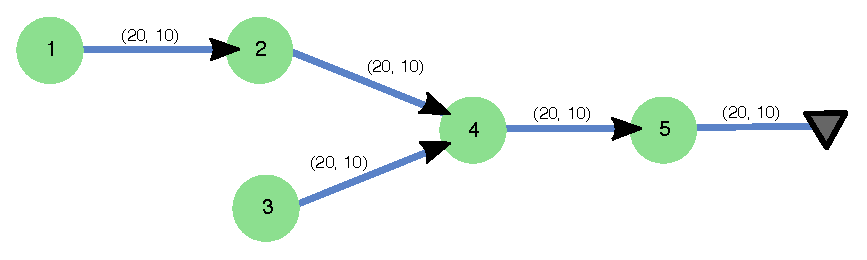
\includegraphics[width=\textwidth]{network.eps}
	\label{fig1}
	\caption{Network of 5 nodes being used to evaluate the performance of both problem formulations.}
\end{figure}

Both the problem formulations are evaluated in the same network to compare the performance of system. 

\subsection{Centralized Control}

\section{Appendix}
\bibliographystyle{unsrt}  
\bibliography{references}  %%% Remove comment to use the external .bib file (using bibtex).

\end{document}
